\documentclass[twocolumn, a4j]{article}
\usepackage{multirow}
\usepackage{amsmath,amssymb}
\usepackage[T1]{fontenc}
\usepackage[dvipdfmx]{graphicx}

\title{「倫理ある商取引ゲーム」において\\不正を抑制するインセンティブ設計の提案}
\renewcommand{\thefootnote}{\fnsymbol{footnote}}
\author{Nozomu Miyamoto\footnotemark[2] nontan@sfc.wide.ad.jp}
\renewcommand{\thefootnote}{\arabic{footnote}}
\date{\today}

\begin{document}

\twocolumn[
\begin{@twocolumnfalse}
  \maketitle
  \vspace{-6mm}
  \begin{abstract}
    先学期の研究では「商取引ゲーム」において不正を防止するインセンティブ設計が不可能であることが証明された.しかしながら,この理論上の商取引に反して実社会の商取引では不正にあうのは稀である.我々はその原因が人々が利己的な行動規範に基づいていないためだと考え,そのような行動規範を倫理と定義し、それに従うプレイヤーのみで行われる「商取引ゲーム」を「倫理ある商取引ゲーム」とした.本研究では,この「倫理ある商取引ゲーム」において不正を防止するインセンティブ設計の手法を提案し,「倫理ある商取引ゲーム」と「商取引ゲーム」の両方でその手法を実験・評価する.実験方法には改善の余地があるものの,初期で誠実なエージェントが一定数以上いる場合に「商取引ゲーム」で不正を抑制することが可能であることがわかった.
  \end{abstract}
  \vspace{2mm}
\end{@twocolumnfalse}
]

\renewcommand{\thefootnote}{\fnsymbol{footnote}}
\footnotetext[2]{慶應義塾大学 環境情報学部 NECO Lab.}
\renewcommand{\thefootnote}{\arabic{footnote}}


\section{はじめに}
インターネットと電子送金の普及によって,国境を超えたグローバルな商取引が瞬時に行えるようになり,我々は日々の生活の中でそれを当然のように受け入れている.また,同時に我々は,国内での電子商取引がそうであったように,このグローバルな商取引でもエスクローサービスと呼ばれる,代金を一時的に預かり商品到着を確認後に支払いを行うサービスを用いることで,詐欺などの不正行為を防止できると信じている.しかしながら,実際のところ,これはエスクローサービスのような商取引の仲介者と別の商取引を結んでいいるに過ぎず,仲介者が信頼できるという前提のもとで成り立っている.\\
 仲介者が信頼できるという前提は,次節で述べる,「第3者に依存しない仲介システム」が存在しているという仮定の上で成り立つものである.また,3節で述べるが,この仮定は,システムから商取引において不正行為を行った当事者が$seller$か$buyer$のどちらであるかを観察できないことを意味している.それ故に,第3者に依存せずに契約での不正行為を防止するシステムは,当事者のうちどちらが不正行為を行ったかという情報を用いずに,当事者達が不正行為を行わないインセンティブ設計を行わなければならない.\\
 本研究の目的は,実社会の商取引において,どのようにして不正行為が抑制されているのかのメカニズムを解明することである.エスクローサービスが電子商取引においては機能しないという前提の上で,電子商取引における不正行為の防止のメカニズムを提案する研究\cite{Shigeo 2000}は存在するものの,暗黙的に商取引の仲介者への信頼が前提となっており,本質的な解決には至っていない.\\
 本稿では,先の条件を満たすシステムを「商取引システム」と呼び,このシステムから参加者達($players$)の通貨の保有量を観察,操作することで商取引のインセンティブ設計を行うものとする.そして,この「商取引システム」を仲介とする商取引を,ゲーム理論を用いて「商取引ゲーム」として定義する.その上で,この「商取引ゲーム」の当事者である$seller$と$buyer$が不正行為を行わないようなインセンティブ設計がシステムから不可能であることを証明し,「商取引ゲーム」において不正行為防止が不可能であることを示す.最後に,今後の研究のため,この理論上の商取引と実社会の商取引を比較することで,なぜ実社会の商取引では不正行為が抑制されているのかを考察する.\\

\section{背景}
\subsection{「第3者に依存しない仲介システム」の必要性}
   商取引において不正行為を防止するためには,第3者に依存せずに動作の正当性が保証された商取引を仲介するシステムが存在していて,かつ,そのシステムは商取引で不正行為を防止できるインセンティブ設計を行える必要がある.仮に第3者に依存せずに動作の正当性が保証された仲介するシステムが存在しないとすれば,再帰的に,商取引を仲介するシステムの動作の正当性を保証する他の仲介するシステムが必要となるため,一向にそのシステムの正当性は保証されない.それ故,必ず第3者に依存せずに動作の正当性が保証された仲介するシステムが存在している必要がある.その上で,商取引において不正行為を防止するには,そのシステムから商取引の当事者達が不正行為を行わなくなるようなインセンティブ設計を行う必要がある.つまりは,第3者に依存せずに動作の正当性が保証されたシステム(本稿では,これを「第3者に依存しない仲介システム」と呼ぶ.)が存在しており,この「第3者に依存しない仲介システム」から商取引の不正行為防止のためのインセンティブ設計が行えなければならない.

\subsection{「行動観測不可の条件」}
仮にこのようなシステムが存在していたとして,このシステムからインセンティブ設計を行う際には,商取引の当事者である$seller$と$buyer$の行動を観察することができないという条件(以後,「行動観察不可の条件」と呼ぶ.)をおくべきである.なぜなら,商取引が失敗した場合に$seller$と$buyer$のどちらに非があるかを確かめるには,第3者に依存せずに動作の正当性が保証されているという前提に反して,誰かしらの第3者に依存する必要があるからである.

例えば,りんごの売買契約を結んだ$seller$と$buyer$がいて,どちらかがシステムにその商取引の失敗を報告したとする.ここで$seller$と$buyer$のどちらが不正行為を行ったかを知るために,代理人を選出して調査を行うことや,りんごにシステムから不正行為を検知するためのセンサーをあらかじめ埋め込むなどの方法がある.しかし,どちらも代理人やセンサーの正当性を保証する製造者などの第3者に依存してしまう.また,代理人や製造者が正当性が保証されたシステムの一部であると仮定しても,第3者である彼らの正当性が保証されているためには,別の「第3者に依存しない仲介システム」を用いて彼らと商取引を結んでいなければならず,その仮定は別の「第3者に依存しない仲介システム」という第3者に依存していることを前提としてしまう.

つまり,商取引において不正行為を防止するためには,「行動観察不可の条件」を満たす「第3者に依存しない仲介システム」が存在していなければならないのである.

\section{「商取引システム」}
 この「行動観察不可の条件」を満たす「第3者に依存しない仲介システム」が存在するのかを論じるために,このシステムに以下の条件を付随したものを「商取引システム」と定義する.
\begin{itemize}
  \item このシステム内には通貨が存在している.
  \item このシステムからは各$player$(システムの参加者)の通貨の保有量を観察・操作することができる.
  \item このシステムを仲介として商取引を行う際,支払いはシステム内の通貨で行われる.
  \item このシステムは商取引の当事者(本稿では$buyer$)から結果の報告を受けた際に各$player$の通貨の保有量を任意に操作する.
\end{itemize}

\section{「商取引ゲーム」}
 また,この「商取引システム」において,商取引で不正行為を防止できるインセンティブ設計を行うことができるのかを検証するするために,このシステムを商取引の仲介として用いる「商取引ゲーム」を次のように定義する.なお,ここでのゲームの$players$(システムの参加者達)は合理的に(期待利得の最も高い)戦略を決定するものとする.

\subsection{ゲームの進め方}
 本稿での商取引は,以下の4つのステップで$seller$と$buyer$が交互に行動を展開するものとする.

\begin{description}
  \item[step1] $seller$は商品$goods$とその価格を告知する
  \item[step2]  その商品の購入を希望する$buyer$が「商取引システム」に商取引の合意を報告する.
  \item[step3]  $seller$は「正当な行為」と「不正な行為」のどちらかの行動選択をする.ここで「正当な行為」を行った場合,$buyer$は契約通りの$goods$を受け取れ, 「不正な行為」を行った場合,$buyer$は契約通りの$goods$を受け取れないものとする.
  \item[step4]  $buyer$は商取引の「成功」か「失敗」かを「商取引システム」に報告する.この報告に基づき,「商取引システム」は$ seller$と$ buyer$の保有する通貨の量を調整する.
\end{description}

\subsection{ゲーム木}
 先の商取引ゲームをゲームの木を用いて表すと図\ref{gametree}のようになる.\textbf{step1}と\textbf{step2}の時点では商取引の結果が変化することはなく,\textbf{step3}で$seller$が「正当な行為」をとるか否かと,\textbf{step4}での$buyer$からの報告によってのみ商取引の結果は変化する.また,「商取引システム」からは「行動観察不可の条件」より$seller$と$buyer$がどの行動をとったかはわからないため,\textbf{step4}での$buyer$の報告にのみ基づいて$seller$と$buyer$の保有する通貨の量を調整しなければならない.つまりは商取引の結果①と③,②と④はそれぞれ$goods$を除く利得は同じでなくてはならない.

\begin{figure*}[b]
  \centering
  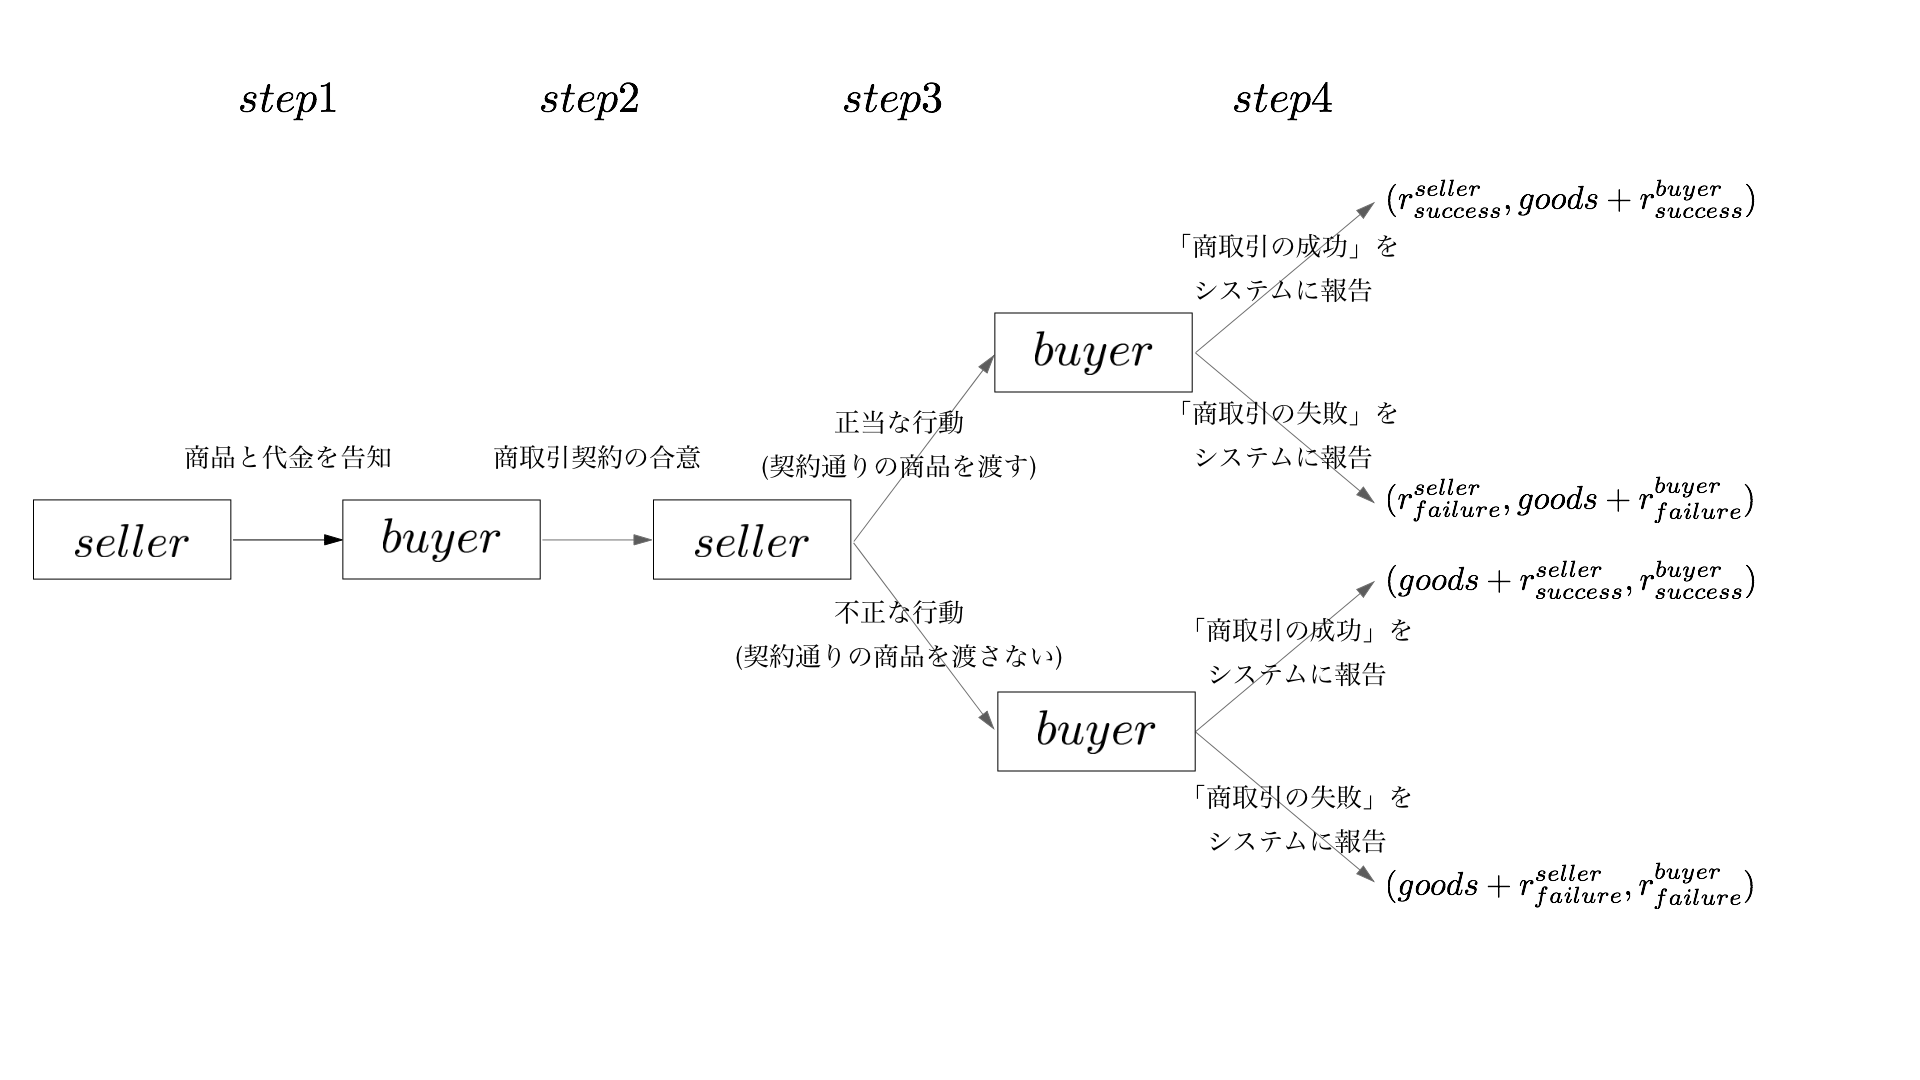
\includegraphics[width=1\linewidth]{gametree.png}
  \caption{「商取引ゲーム」のゲーム木}
  \label{gametree}
\end{figure*}

また,この商取引のモデルは,第3ステップ以降の$seller$の行動選択と,それに対する第4ステップの$ buyer$の行動選択を,非協力戦略型ゲームとしてとらえられる.ここで,戦略$ s^{player}_{n}$を$ player$(ここでは$seller$か$buyer$)の取りうる戦略番号$n$の戦略として,$seller$と$buyer$のそれぞれの戦略は以下のように定義する.\\

\begin{description}
  \item[$s^{seller}_1$]… 正当な行為を行う
  \item[$s^{seller}_2$]… 不正な行為を行う
  \item[$s^{buyer}_1$]… $ seller$が正当な行為を行った場合は「成功」を,不正な行動を行った場合は「失敗」を報告する
  \item[$s^{buyer}_2$]… $ seller$が正当な行為を行った場合は「成功」を,不正な行動を行った場合は「成功」を報告する
  \item[$s^{buyer}_3$]… $ seller$が正当な行為を行った場合は「失敗」を,不正な行動を行った場合は「失敗」を報告する
  \item[$s^{buyer}_4$]… $ seller$が正当な行為を行った場合は「失敗」を,不正な行動を行った場合は「成功」を報告する
\end{description}

\subsection{非協力戦略型ゲーム}
\newcommand{\successseller}{
  \begin{tabular}{c}
    $(r^{seller}_{success},$\\
    $goods+r^{buyer}_{success})$
  \end{tabular}
}
\newcommand{\successbuyer}{
  \begin{tabular}{c}
    $(goods+r^{seller}_{success},$\\
    $r^{buyer}_{success})$
  \end{tabular}
}
\newcommand{\fseller}{
  \begin{tabular}{c}
    $(r^{seller}_{failure},$\\
    $goods+r^{buyer}_{failure})$
  \end{tabular}
}
\newcommand{\fbuyer}{
  \begin{tabular}{c}
    $(goods+r^{seller}_{failure},$\\
    $r^{buyer}_{failure})$
  \end{tabular}
}

\begin{table*}[b]
\begin{tabular}{|l|l|l|l|l|l|}
\hline
\multicolumn{2}{|l|}{\multirow{2}{*}{}} & \multicolumn{4}{l|}{$buyer$} \\ \cline{3-6}
\multicolumn{2}{|l|}{}                  &$s^{buyer}_1$&$s^{buyer}_2$&$s^{buyer}_3$&$s^{buyer}_4$\\ \hline
\multirow{2}{*}{$seller$}
&$s^{seller}_1$&\successseller&\successseller&\fseller&\fseller\\ \cline{2-6}
&$s^{seller}_2$&\fbuyer&\successbuyer&\fbuyer&\successbuyer\\ \hline
\end{tabular}
\caption{非協力戦略型ゲームとして表した「商取引ゲーム」の利得表}
\label{gametable}
\end{table*}

また,この商取引のモデルは,第3ステップ以降の$seller$の行動選択と,それに対する第4ステップの$ buyer$の行動選択を,非協力戦略型ゲームとしてとらえられる.ここで,戦略$ s^{player}_{n}$を$ player$(ここでは$seller$か$buyer$)の取りうる戦略番号$n$の戦略として,$ seller$と$ buyer$のそれぞれの戦略は以下のように定義する.\\

\begin{description}
  \item[$s^{seller}_1$]… 正当な行為を行う
  \item[$s^{seller}_2$]… 不正な行為を行う
  \item[$s^{buyer}_1$]… $ seller$が正当な行為をとった場合は「成功」を,不正な行動をとった場合は「失敗」を報告する
  \item[$s^{buyer}_2$]… $ seller$が正当な行為をとった場合は「成功」を,不正な行動をとった場合は「成功」を報告する
  \item[$s^{buyer}_3$]… $ seller$が正当な行為をとった場合は「失敗」を,不正な行動をとった場合は「失敗」を報告する
  \item[$s^{buyer}_4$]… $ seller$が正当な行為をとった場合は「失敗」を,不正な行動をとった場合は「成功」を報告する
\end{description}

\subsection{不正防止の不可能性}
2018年度秋学期の研究により,「商取引ゲーム」において不正を防止するインセンティブ設計が不可能であることが示された.

\section{「倫理ある商取引ゲーム」}
% 「不正防止の不可能性」より,「商取引ゲーム」においては不正を防止するインセンティブ設計ができないことがわかった.しかし,この理論上の商取引に反して,実社会の商取引においては不正行為がある程度抑制されている.これは実社会の商取引を行う人々が,自身の利益を最大化するような利己的な行動規範に従って戦略を選んでおらず,完全な「商取引ゲーム」を行っていないためだからだと考えられる.そこで本稿では,この利己的でない行動規範を「倫理」とし,「倫理」に従うプレイヤーのみで行われる「商取引ゲーム」を「倫理ある商取引ゲーム」とすることで,この「倫理ある商取引ゲーム」において不正を防止するインセンティブ設計が可能であることを示す.

\subsection{倫理}
「不正防止の不可能性」より,「商取引ゲーム」においては不正を防止するインセンティブ設計ができないことがわかった.しかし,この理論上の商取引に反して,実社会の商取引においては不正行為がある程度、抑制されている.これは実社会の商取引を行う人々が,自身の利益を最大化するような利己的な行動規範に従って戦略を選んでおらず,完全な「商取引ゲーム」を行っていないためだと考えられる.本稿では、実社会の商取引において「泣き寝入り」と呼ばれるような$buyer$が不正にあった場合に「成功」を報告する戦略があまり取られていないことに着目し、$buyer$が不正にあった場合に必ず「失敗」を報告する行動規範を倫理として定義し、この倫理に従うプレイヤーのみで行われる「商取引ゲーム」を「倫理ある商取引ゲーム」とする.

% 「不正防止の不可能性」より,「商取引ゲーム」においては不正を防止するインセンティブ設計ができないことがわかった.しかし,この理論上の商取引に反して,実社会の商取引においては不正行為がある程度抑制されている.これは実社会の商取引を行う人々が,自身の利益を最大化するような利己的な行動規範に従って戦略を選んでおらず,完全な「商取引ゲーム」を行っていないためだと考えられる.そこで、本稿ではそのような行動規範を倫理と定義し、利己的な行動規範との違いについて論じる.

% 利己的な行動規範とは,相手が各戦略をとる主観的な確率とその際の自身の利得から自身の各戦略の期待利得を算出し,それが高い方の戦略を選択する行動規範である.各利得は「商取引システム」から一意に決定されるため,「倫理」と利己的な行動規範の差異は相手が各戦略をとる主観的な確率にあると考えられる.つまりは相手が特定の戦略をとる確率を通常よりも低く(もしくは高く)見積もっていることになる.そのため倫理が具体的にどのように利己的な行動規範と違うのかを知るためには、$seller$と$buyer$のとりえる各戦略について考える必要がある.
%
% 「商取引ゲーム」においては$seller$の戦略は2通りあり$buyer$の戦略は4通りあった.これらの戦略は「$seller$が商品を渡すか否か」と「$buyer$が商品の受け取りを報告するか否か」,「$buyer$が不正にあった場合に告発するか否か」の3つの観点から2分できる.そこで,それらの観点で2分した片方の戦略群を相手が選ぶ可能性が0であるとした場合について考える.また,この主観的な確率が0であるとみなす戦略をそのプレイヤーはとりえないものとして考える.本稿では、実社会の商取引において「泣き寝入り」と呼ばれるような戦略があまり取られていないことに着目し、$buyer$が不正にあった場合に必ず「失敗」を報告する行動規範を倫理として定義する.

\subsection{倫理ある商取引ゲーム}
「倫理ある商取引ゲーム」においては$buyer$は$seller$が不正を行った場合にかならず「失敗」を報告するためゲーム木はFigure\ref{ethical-gametree}のようになる.また、同様に$buyer$が戦略$s^{buyer}_2, s^{buyer}_4$を取らないため、非協力戦略型ゲームの表はTable\ref{ethical-gametable}のようになる.


% まず「$seller$が商品を渡すか否か」について考察する.プレイヤーが$seller$の「商品を渡す」という戦略を取りえない行動規範に従って戦略を選ぶとき「商取引ゲーム」は必ず失敗する.また,プレイヤーが「商品を渡さない」という戦略を取り得ない行動規範に従って戦略を選ぶとき,「商取引ゲーム」を成功させるインセンティブ設計は可能になるが,これは「プレイヤーが不正を起こさないから成功する」というようなものである.
% 次に「$seller$が商取引契約を履行した場合に$buyer$が『成功』を報告するか否か」については,$buyer$が「$seller$が履行した場合に『失敗』を報告する」戦略をとる「商取引ゲーム」では誠実な戦略組をとり得ることはなく,$buyer$が「$seller$が商取引契約を履行した場合に『成功』を報告する」戦略をとるなら,必ず$seller$は商取引契約を反故にするだろう.
% 最後に「$seller$が商取引契約を反故にした場合に$buyer$が『成功』を報告するか否か」について,$buyer$が$seller$が商取引契約を反故にした場合に必ず『成功』を報告するなら,$seller$は必ず商取引契約を反故にするだろう.残るは「$seller$が商取引契約を反故にした場合に必ず『失敗』を報告する」場合である.この場合のときのみ,$seller$は商取引契約を履行するか反故にするかの選択を商品価値$goods$と取引失敗時のシステムによって調整される利得$r^{seller}_{failure}$によって判断することとなる.
%
% そのため,これまでの6パターンのなかで,この「$seller$が商取引契約を反故にした場合に必ず『失敗』を報告する」という行動規範がもっとも考えられる.また,これは実社会の商取引において,多くの場合で不正に会った場合にそれを告発していることから考えるに妥当な条件である.そこで本稿では「$seller$が商取引契約を反故にした場合に必ず『失敗』を報告する戦略をとり,相手がそれ以外の戦略とる確率を0とみなすプレイヤーを倫理あるプレイヤーとして定義する.また,この倫理に従うプレイヤーのみが参加する「商取引ゲーム」を「倫理ある商取引ゲーム」とする.

\clearpage

\begin{figure*}[b]
  \centering
  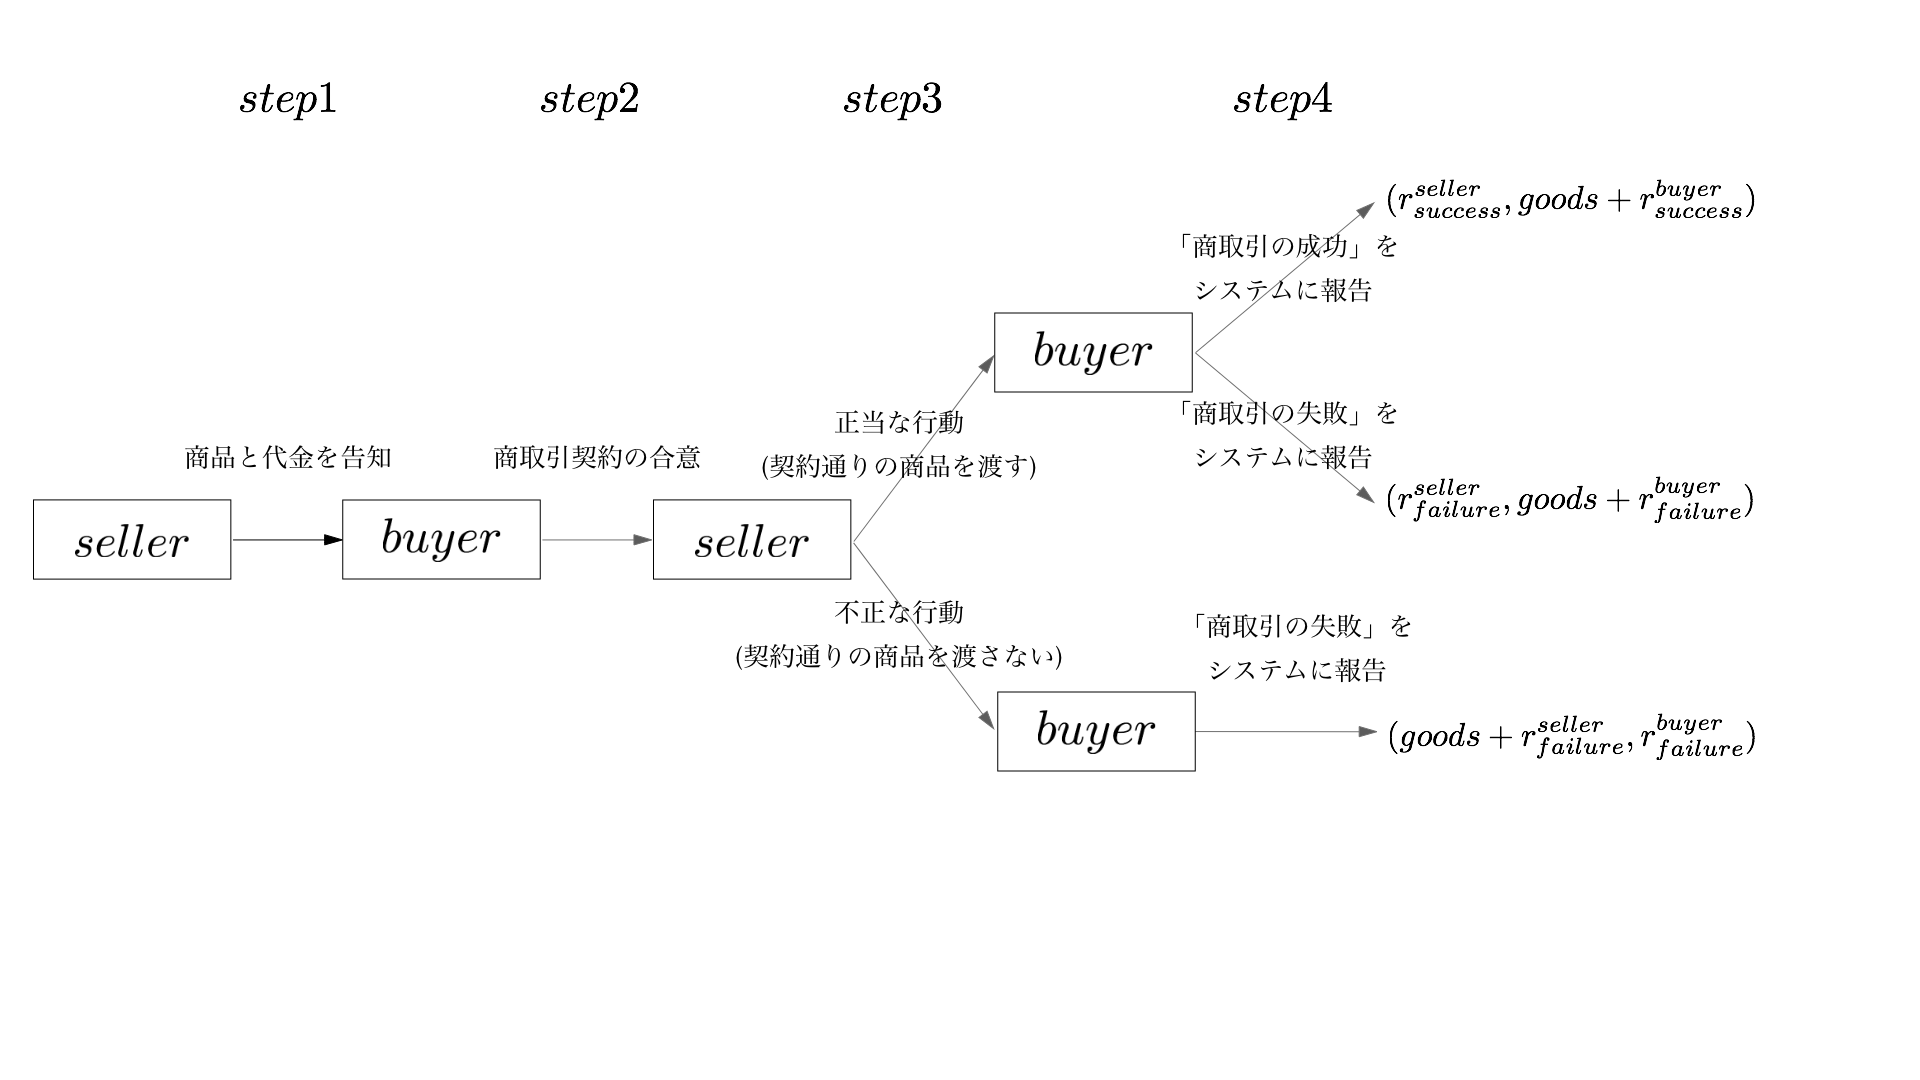
\includegraphics[width=1\linewidth]{ethical-gametree.png}
  \caption{「倫理ある商取引ゲーム」のゲーム木}
  \label{ethical-gametree}
\end{figure*}


\begin{table*}[b]
\centering
\begin{tabular}{|l|l|l|l|}
\hline
\multicolumn{2}{|l|}{\multirow{2}{*}{}} & \multicolumn{2}{l|}{$buyer$} \\ \cline{3-4}
\multicolumn{2}{|l|}{}                  &$s^{buyer}_1$&$s^{buyer}_3$\\ \hline
\multirow{2}{*}{$seller$}
&$s^{seller}_1$&\successseller&\fseller\\ \cline{2-4}
&$s^{seller}_2$&\fbuyer&\fbuyer\\ \hline
\end{tabular}
\caption{非協力戦略型ゲームとして表した「倫理ある商取引ゲーム」の利得表}
\label{ethical-gametable}
\end{table*}

\onecolumn

\subsection{誠実な戦略が取られた割合と報告された成功率の関係}
この「倫理ある商取引ゲーム」においては,商取引が失敗した場合に必ず「失敗」が報告されるため,商取引の成功率は「商取引システム」に「成功」が報告された割合以上である.ここで任意の$ player $が任意の$ opportunity $と過去に「商取引ゲーム」を行った際,誠実な戦略($ s^{seller}_1, s^{buyer}_1 $のいずれか)をとってきた割合を$ HonestStrategyRate(player, opportunity) $とし,同様に報告された商取引の成功率を$ ReportedSuccessRate(player, opportunity) $とする.そのとき,$ HonestStrategyRate(player, opportunity) $と$ ReporttedSuccessRate(player, opportunity) $の関係は次の式で表せる.


\begin{equation}
  HonestStrategyRate(player, opportunity) \geq ReportedSuccessRate(player, opportunity)
\end{equation}

\subsection{自己信頼}
ここで$ HonestStrategyRate(player, player) $と$ ReportedSuccessRate(player, player) $は1とする.これは$ player $が$ player $自身と行う商取引は必ず成功するためである.

\subsection{将来期待利得}
通常の「商取引ゲーム」においては誠実な戦略を取ってきた割合と報告された商取引ゲームの成功率の間の関係性はわからないため,繰り返しゲームと考えても次のゲームへ引き継げる情報がなかったため将来期待利得を考慮しなかったが,「倫理ある商取引ゲーム」においては先に述べた関係式が得られるため,将来期待利得を考慮する必要がある.商取引で「成功」が報告された場合の$ seller $と$ buyer $の将来期待利得を$ \epsilon^{seller}, \epsilon^{seller} $とし,「失敗」が報告された場合の将来的な期待利得を$ \lambda^{seller}, \lambda^{buyer} $とおくと,「倫理ある商取引ゲーム」のゲーム木と非協力戦略型ゲームの表は次のように書き換えられる.
また,本稿では,これらについて$ \epsilon^{player} > \lambda^{player} $と仮定する.

\section{不正が防止される条件}
\subsection{不正が抑制される戦略組と期待利得の不等式}
「倫理ある商取引ゲーム」において不正が生じないためには$seller$と$buyer$の戦略組を$(s^{seller}_1, s^{buyer}_1)$に帰着させなくてはならない.
そのためには$seller$が戦略$s^{seller}_1$をとった場合の期待利得$E(r|s^{seller}_1)$が戦略$s^{seller}_2$をとった場合の期待利得$E(r|s^{seller}_2)$より大きく,$buyer$が戦略$s^{buyer}_1$をとった場合の期待利得$E(r|s^{buyer}_1)$が戦略$s^{buyer}_3$をとった場合の期待利得$E(r|s^{buyer}_3)$より大きくならなければならない.
つまりは,$E(r|s^{seller}_1) > E(r|s^{seller}_2)$かつ$E(r|s^{buyer}_1) > E(r|s^{buyer}_3)$を満たす$(r^{seller}_{success}, r^{seller}_{failure}, r^{buyer}_{success}, r^{buyer}_{failure})$の組を「商取引システム」から決定できる必要がある.

\subsection{$ seller $と$ buyer $の期待利得}

$ seller $と$ buyer $の各戦略の利得の期待値は以下のように表せる.\\


$ E(R|s^{seller}_1) = p^{buyer}_1 (r^{seller}_{success} + \epsilon^{seller}) + p^{buyer}_3 (r^{seller}_{failure} + \lambda^{seller}) $ \\

$ E(R|s^{seller}_2) = p^{buyer}_1 (goods + r^{seller}_{failure} + \lambda^{seller}) + p^{buyer}_3 (goods + r^{seller}_{failure} + \lambda^{seller}) $ \\

$ = goods + r^{seller}_{failure} + \lambda^{seller} $ \\

$ \because p^{buyer}_1 + p^{buyer}_3 = 1 $($ buyer $が$ p^{buyer}_2 $と$ p^{buyer}_4 $が0と見積もられているため) \\

$ E(R|s^{buyer}_1) = p^{seller}_1 (goods + r^{buyer}_{success} + \epsilon^{buyer}) + p^{seller}_2 (r^{buyer}_{failure} + \lambda^{buyer}) $ \\

$ E(R|s^{buyer}_3) = p^{seller}_1(goods+r^{buyer}_{failure} + \lambda^{buyer}) + p^{seller}_2 (r^{buyer}_{failure} + \lambda^{buyer}) $ \\

$ = p^{seller}_1 goods + r^{buyer}_{failure} + \lambda^{buyer} $ \\

$ \because p^{seller}_1 + p^{seller}_2 = 1 $ \\


\subsection{$ seller $が誠実な戦略をとる条件}

$ E(R|s^{seller}_1) > E(R|s^{seller}_2) $
$ \therefore p^{buyer}_1 (r^{seller}_{success} + \epsilon) + p^{buyer}_2 (r^{seller}_{failure} + \lambda) > goods + r^{seller}_{failure} + \lambda $
$ \therefore p^{buyer}_1(r^{seller}_{success} + \epsilon) - p^{buyer}_1(r^{seller}_{failure} + \lambda) > goods $
$ \therefore p^{buyer}_1(r^{seller}_{success} - r^{seller}_{failure} + \epsilon - \lambda) > goods $
仮定より,$ \epsilon > \lambda $のため,
$ p^{buyer}_1 (r^{seller}_{success} - r^{seller}_{failure}) \geq goods $を満たせばよい.

$ 0 < p^{buyer}_1 $を仮定するならば,
$ r^{seller}_{success} - r^{seller}_{failure} \geq \frac{goods}{p^{buyer}_1} $


\subsection{$ buyer $が誠実な戦略をとる条件}

$ E(R|s^{buyer}_1) > E(R|s^{buyer}_3) $
$ \therefore p^{seller}_1 (goods + r^{buyer}_{success}) + p^{seller}_2 r^{buyer}_{failure} > p^{seller}_1(goods+r^{buyer}_{failure}) + p^{seller}_2 r^{buyer}_{failure} $
$ \therefore p^{seller}_1(r^{buyer}_{success} - r^{buyer}_{failure}) > 0 $
$ 0 < p^{seller}_1 $を仮定するならば,
$ r^{buyer}_{success} - r^{buyer}_{failure} > 0 $

上記をまとめると,$ 0<p^{buyer}_1 $かつ $ 0 < p^{seller}_{1} $を仮定した上で,
$ r^{seller}_{success} - r^{seller}_{failure} \geq \frac{goods}{p^{buyer}_1} $かつ$ r^{buyer}_{success} - r^{buyer}_{failure} > 0 $
を満たせば,「倫理ある商取引ゲーム」では不正を抑制することができる.


\subsection{相手の誠実さ $ P^{player} $}

ここで,任意の$ player $が誠実な戦略($ p^{seller}_1, p^{buyer}_1 $のいづれか)をとる主観確率を$ p^{player}_1 $とすると,$ p^{player}_1 $は各プレイヤーに対して誠実な戦略をとった割合$ HonestyStrategyRate(player, opportunity) $と任意の重み$ r.w.^{player} $を用いて次のように表せる.
$ p^{player}_1 \equiv \sum^{players}_{opotunity} r.w.^{opotunity} HonestyStrategyRate(player, opotunity) $


\subsection{最低信頼度 $ T^{player} $}

ただ「商取引システム」からは$ HonestyStrategyRate $がわからないため,これでは$ p^{player}_1 $を求めることができない.そこで$ HonestyStrategyRate $の代わりに$ ReportedSuccessRate $を用いて同様の$ r.w.^{player} $で重み付けした総和を最低信頼度$ T^{player} $とおくことにする.

$ T^{player} \equiv \sum^{players}_{opotunity} {r.w.}^{opotunity} ReportedSuccessRate(player, opotunity) $

ここで$ HonestyStrategyRate \geq ReportedSuccessRate $であるため,$ p^{player}_1 \geq T^{player} $がいえる.

それゆえに,
$ r^{seller}_{success} - r^{seller}_{failure}  \geq \frac{goods}{T^{buyer}} \geq \frac{goods}{p^{buyer}_1} $
となる.
ここから「倫理ある商取引ゲーム」において不正が抑制される条件は次のように書き直せる.

$ 0<p^{buyer}_1 $かつ $ 0 < p^{seller}_{1} $を仮定した上で,
$ r^{seller}_{success} - r^{seller}_{failure} \geq \frac{goods}{T^{buyer}} $かつ$ r^{buyer}_{success} - r^{buyer}_{failure} > 0 $

つまりは,この最低信頼度$ T^{player} $をもちいることで,以下の条件を満たす$ (r^{seller}_{success}, r^{seller}_{failure}, r^{buyer}_{success}, r^{buyer}_{failure}) $の組を決定できる.


\section{提案手法}
「倫理ある商取引ゲーム」においては,最低信頼度$ T^{player} $を用いた上記の条件式を満たせば,不正を防止することが可能になる.ただ,上記の条件のみでは「商取引システム」から保有通貨の変化量の組$ (r^{seller}_{success}, r^{seller}_{failure}, r^{buyer}_{success}, r^{buyer}_{failure}) $を一意に決定できないので,いくつかの条件を追加する.


\subsection{取引成功前後の残高の変化}
商取引成功前後では$ buyer $は商品$ goods $の価格$ price $だけ残高が減り$ seller $は$ price $だけ残高が増えるものとする.そのため商取引前後では$ seller $と$ buyer $の残高の合計は変化しない.ここから,$ r^{seller}_{success} $と$ r^{buyer}_{success} $は以下のように記せる.

$ r^{seller}_{success} = price $
$ r^{buyer}_{success} = -price $
$ r^{seller}_{success} + r^{buyer}_{succcess} = 0 $

\subsection{エスクロー係数 E}
まずは「失敗」が報告された時に$ seller $と$ buyer $から失われる通貨の量の合計を$ EscrowCost $とおいて考え,同時に商品価格$ price $にエスクロー係数$ E $を掛けたものとする.(ここで$ price $は$ goods $の価格である)

$ EscrowCost \equiv (r^{buyer}_{success} - r^{buyer}_{failure}) + (r^{seller}_{success} - r^{seller}_{failure}) $
$ = E \cdot price $

\subsection{負担比率}
ここで問題となるのは$ EscrowCost $を求めるための$ seller $と$ buyer $の負担比率をどのようにして決定するかである.本稿では最低信頼度$ T^{player} $を用いてこの負担比率を決定することとする.

$ (r^{buyer}_{success} - r^{buyer}_{failure}):(r^{seller}_{success} - r^{seller}_{failure}) = w(T^{buyer}):w(T^{seller}) $

ここで最低信頼度が高い$ player $の方が負担比率が小さくなるように責任比重関数$ w(x) $は値域$ 0 \leq  x \leq 1 $において$ w'(x)>0 $を満たすものとする.

\subsection{責任比重関数$ w(x) $}
本稿では負担比重関数は恒等写像$ w(x)=x $とする.

\subsection{ReputationWeights}
最低信頼度$ T^{player} $を求めるにあたって$ r.w.^{opportunity} $を決定する必要がある.$ r.w.^{opportunity} $は誠実さ$ T^{player}_1 $を求める際に$ ReportedSuccessRate(player, opportunity) $に係る任意の重みである.これはつまり任意の$ player $が誠実な戦略をとる主観的確率を考える際に,$ player $と$ opportunity $の間であった過去の商取引での報告された成功率をどの程度信じるかである.仮に$ player $と$ opportunity $の間で信頼関係があれば$ ReportedSuccessRate $は$ 1 $になる.なので「商取引システム」の参加者数$ n $が特定できる場合は$ \frac{1}{n} $が妥当だろう.逆に不特定多数であり,同一の意志によって複数のプレイヤーが動いている場合は,保有している通貨量$ b^{opportunity} $の全体の通貨の総量に占める割合が良いだろう.

$ r.w.^{opportunity} \equiv \frac{b^{opportunity}}{\sum^{players}_{i}b^{i}} $


\subsection{EscrowCostの分配}
「失敗」が報告されたときに失われる$ EscrowCost $は消滅するのではなく参加者に分配する.これは全体の通貨量の減少によって通貨の価値が上がって商品価格が下がるという経済原理が生じ,インセンティブ設計が複雑化するのを防ぐためである.そこで$ EscrowCost $として失われた通貨は任意の重み$ e.w.^{player} (\sum^{players}_{player}e.w.^{player} = 1) $を用いて分配し「商取引ゲーム」の前後で全体の通貨量を等しくする.

\subsection{EscrowWeights}
EscrowCostの分配に関しては「商取引システム」に参加している各プレイヤーの通貨の保有率に応じて分配する.$ seller $と$ buyer $を含んでいるのは,仮に$ seller $と$ buyer $以外のすべてのプレイヤーで分配した場合,$ seller $もしくは$ buyer $は結託する別のプレイヤーに保有する通貨の一部を一時的に預けることで,その分だけ$ EscrowCost $の負担を軽減することが可能になるためである.そこで本稿では任意の重み$ e.w.^{player} $を以下のように定義する.

$ e.w.^{player} \equiv \frac{b^{player}}{\sum^{players}_{escrow}b^{escrow}} $

\subsection{謎の条件}
$ \frac{w(T^{buyer}_1)E \cdot price}{w(T^{buyer}_1) + w(T^{seller}_1)} \geq \frac{price}{T^{buyer}} \geq \frac{goods}{p^{buyer}_1} $

上記の条件式から$ \frac{price}{ T^{buyer} } $でうまくいくはずだったが何故かうまく行かず,$ \frac{price}{ \min(T^{buyer}, T^{seller})} $をもちいたらうまくいったのでこちらを採用することとした.$ p^{buyer} $と$ P^{player}_1 $の関係性に問題があるためだと思われる.

$ \frac{w(T^{buyer}_1)E \cdot price}{w(T^{buyer}_1) + w(T^{seller}_1)} \geq \frac{price}{ \min(T^{buyer}, T^{seller})} $


\subsection{残高の変化量の組$ (r^{seller}_{success}, r^{seller}_{failure}, r^{buyer}_{success}, r^{buyer}_{failure}) $}
上記の条件群を用いて残高の変化量の組$ (r^{seller}_{success}, r^{seller}_{failure}, r^{buyer}_{success}, r^{buyer}_{failure}) $を決定する.


$ r^{seller}_{success}+r^{buyer}_{success} = 0 $

$ r^{seller}_{failure}+r^{buyer}_{failure} = -E \cdot price $

$ r^{seller}_{success} - r^{seller}_{failure} = \frac{w(T^{buyer}_1)E \cdot price}{w(T^{buyer}_1) + w(T^{seller}_1)} \geq \frac{price}{T^{buyer}} $

$ r^{buyer}_{success} - r^{buyer}_{failure} = \frac{w(T^{seller}_1)E \cdot price}{w(T^{buyer}_1) + w(T^{seller}_1)} \geq 0 $

$ \frac{w(T^{buyer})E \cdot price}{w(T^{buyer}) + w(T^{seller})} = \frac{price}{\min(T^{buyer}, T^{seller})} $

$ E $ = $ \frac{w(T^{buyer})+w(T^{seller})}{w(T^{buyer}) \cdot \min(T^{buyer}, T^{seller})} $

$ r^{seller}_{success}-r^{seller}_{failure} = \frac{price}{min(T^{buyer}, T^{seller})} $

$ r^{buyer}_{success} - r^{buyer}_{failure} = \frac{w(T^{seller}) \cdot price}{w(T^{buyer}) \cdot \min(T^{buyer}, T^{seller})} $


$ r^{seller}_{success} = price $
$ r^{buyer}_{success} = -price $
$ r^{seller}_{failure} = price \cdot (1 - \frac{1}{min(T^{buyer}, T^{seller})}) $
$ r^{buyer}_{failure} = - price \cdot (\frac{T^{seller}}{T^{buyer} \cdot \min(T^{buyer}, T^{seller})} + 1) $

\twocolumn

\section{実験方法}
提案手法を用いることで不正が防止されるかどうかを検証するためにコンピューターシミュレーションを用いた実験を行う.この実験では$ (s^{seller_1}, s^{seller}_2) $と$ (s^{buyer}_1, s^{buyer}_2, s^{buyer}_3, s^{buyer}_4) $から任意の戦略組をもつエージェント(全8通り)を10機用意して下記の試行を繰り返す.試行ごとに過去100回分の「真の商取引の成功率(TrueSuccessRate)」と「商取引システム」に「報告された成功率(ReportedSuccessRate)」を記録する.

①10機のエージェントからランダムに$ seller $と$ buyer $を決定し「商取引ゲーム」を行う.
②残高の変化量の組$ (r^{seller}_{success}, r^{buyer}_{success}, r^{seller}_{failure}, r^{buyer}_{failure}) $を算出し,「失敗」が報告された場合に$ seller $と$ buyer $の残高が0未満にならないかを判定する.ここで0未満になる場合は再度,①からやり直し,100回連続で
③$ seller $と$ buyer $のエージェントは戦略から「商取引システム」に報告される結果を決定する.
④「商取引システム」は報告された結果に応じてすべてのエージェントの残高を操作する.
⑤試行回数が10000回になるまで①から④を繰り返す.

\subsection{「 倫理ある商取引ゲーム」での実験}
「倫理ある商取引ゲーム」では$ seller $と$ buyer $がとりえる戦略は$ (s^{seller_1}, s^{seller}_2) $と$ (s^{buyer}_1, s^{buyer}_3 $のみであるため,これらを組み合わせた4パターンのエージェントを全体で10機用意して実験を行う.この10機の4パターンでの構成は268通りあるので,その全て場合で1回づつ実験を行う.

\subsection{「商取引ゲーム」での実験}
「倫理ある商取引ゲーム」では$ seller $と$ buyer $がすべての戦略をとりえるため,8パターンのエージェントを全体で10機用意して実験を行う.この10機の4パターンでの構成は19960通りあるので,モンテカルロ法を用いてランダムに重複ありの1000パターンの構成を生成し実験を行う.

\section{評価}

\begin{figure}[h]
  \begin{tabular}{cc}
    %---- 最初の図 ---------------------------
    \begin{minipage}[t]{1\hsize}
      \centering
      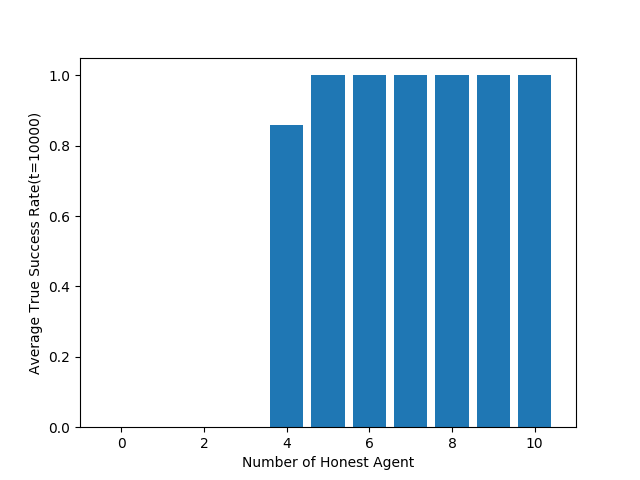
\includegraphics[keepaspectratio, width=1\linewidth]{ethical-aggregate.png}
      \caption{「倫理ある商取引ゲーム」}
      \label{ethical-experiment-aggregate}
    \end{minipage} \\
    %---- 2番目の図 --------------------------
    \begin{minipage}[t]{1\hsize}
      \centering
      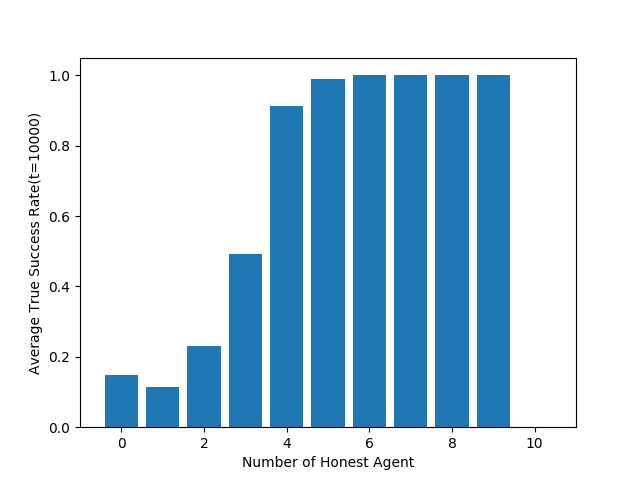
\includegraphics[keepaspectratio, width=1\linewidth]{no-ethical-aggregate.png}
      \caption{「商取引ゲーム」}
      \label{non-ethical-experiment-aggregate}
    \end{minipage}
    % ---- 図はここまで ----------------------
  \end{tabular}
\end{figure}

\subsection{「倫理ある商取引ゲーム」での評価}
「倫理ある商取引ゲーム」における286回の実験データを誠実なエージェントの数ごとに集計し,「商取引ゲーム」を10000万回を繰り返したときの真の成功率の平均をプロットしたのがFigure\ref{ethical-experiment-aggregate}である.誠実なエージェントが3機以下の場合は真の商取引の成功率の平均はいずれも0\%であったが,5機以上の場合はいずれも100\%に収束していた.

\subsection{「商取引ゲーム」での評価}
同様に,通常の「商取引ゲーム」における1000件の実験データを誠実なエージェントの数ごとに集計し,「商取引ゲーム」を10000万回を繰り返したときの真の成功率の平均をプロットしたのがFigure\ref{non-ethical-experiment-aggregate}である.こちらも誠実なエージェントが5機以上の場合は真の商取引の成功率の平均はいづれも99\%を超えていた.また,「倫理ある商取引ゲーム」での実験に比べて4機の場合に比べてこちらの方が真の商取引の成功率の平均は高かく,3機以下の場合でも完全に0\%にはならなかった.

\section{考察}
「倫理ある商取引ゲーム」において誠実なエージェントが1体以下の場合,どの2体のエージェントで「商取引ゲーム」を行っても商取引は失敗する.そのため誠実なエージェントが1体以下の場合に商取引の成功率が0\%になるのは納得である.しかし,今回の実験では2体もしくは3体の場合でも真の商取引の成功率の平均が0\%になっている.この点は疑問である.また,今回のインセンティブ設計のアルゴリズムは「倫理ある商取引ゲーム」を前提としているにも関わらず,通常の「商取引ゲーム」の方が誠実なエージェントが4体のときの真の商取引の成功率の平均値が高いのは不可解である.これらの原因としては,確率的な試行であるにも関わらず「倫理ある商取引ゲーム」においては286パターンのエージェントの構成で1回づつしかサンプリングを行っていないことや,エージェントの構成が19960パターン考えられる通常の「商取引ゲーム」で1000回しか試行をしていないことなどが原因として考えられる.また,最低信頼度$T^{player}$と誠実さ$P^{player}_1$の関係性が$p^{buyer}_1$との関係性とすり替わっていることも原因として考えられる.実験方法やインセンティブ設計を修正する必要があると思われる.現状の結果から唯一いえることがあるとすれば,誠実なエージェントの割合が一定を超えると「商取引ゲーム」の不正行為が防止できるということである.


\section*{謝辞}
 所属する研究会である慶應SFC村井研NECO Lab.の指導教員の斉藤賢爾氏と入会時よりお世話になっている阿部涼介氏,及び,今学期のKGLをなさっていた菅藤佑太氏,そのほかNECO lab.の方々への感謝をここに記します.

\renewcommand{\refname}{参考文献}
\begin{thebibliography}{数字}
  \bibitem[Shigeo 2000]{Shigeo 2000} Shigeo Mastubara and Makoto Yoko, Fraud-Free Exchange Mechanisms in Electronic Commerce, Journal of Japanese Society for Artificial Intelligence(2000).
\end{thebibliography}

\end{document}
